\chapter{Нейросетевой алгоритм контроля качества рентгеновских снимков грудной клетки в задаче диагностики туберкулёза лёгких}\label{ch:ch3}

Согласно клиническим рекомендациям Минздрава России, одним из первых этапов выявления и диагностики туберкулёза лёгких является рентгенофлюорографическое исследование~\cite{васильева2022туберкулез}. При этом в последние годы в практику внедряются компьютерные системы автоматической обработки медицинских данных и диагностики заболеваний на основе искуственного интеллекта, в том числе для в категории флюорографии~\cite{СМ106054, рг2023, рбк2023, интерфакс2023}.

Одной из актуальных задач при применении методов глубокого обучения в медицинской диагностике является анализ и предобработка входных данных. Необходим контроль соответствия входной информации и применяемого обученного (обучаемого) метода глубокого обучения. Это, например, требуется при контроле наличия адверсативных атак на данные~\cite{finlayson2019adversarial}.

Контроль качества рентгеновских снимков грудной клетки на основании разных параметров важен для полноценного анализа снимка и постановки правильного диагноза. Автоматическое определение контроля пространственных условий снимка (позы пациента, положения грудной клетки в кадре и т.п.) рассматривается в работах~\cite{nousiainen2021automating, von2020robust, jia2019application}. В работе~\cite{sadre2021validating} изучено влияние качества снимка на результаты автоматической диагностики COVID"~19.

В данной главе контроль входных рентгеновских снимков используется для проверки соответствия уровня облучения снимка уровню, требуемому для качественной диагностики туберкулёза лёгких. Рассматриваются:
\begin{enumerate}[beginpenalty=10000]
	\item задача автоматического определения уровня жёсткости рентгеновского снимка грудной клетки с помощью нейросетевого алгоритма;
	\item влияние предварительной фильтрации обучающей и валидационной выборок на качество работы алгоритма классификации в задаче диагностики туберкулёза лёгких по рентгеновским снимкам грудной клетки.
\end{enumerate}

Несмотря на то, что использование при анализе рентгенограммы грудной клетки, помимо фронтальной, также и боковой проекции повышает качество анализа, в том числе компьютерного, прирост качества для разных задач разный и далеко не всегда значительный~\cite{kluthke2016additional, hashir2020quantifying}. Кроме того, на практике в подавляющем числе случаев имеются только снимки, сделанные во фронтальной проекции~\cite{вишнякова2016частота}, поэтому в рамках данной главы рассматриваются фронтальные изображения грудной клетки.

\section{Метод оценки жёсткости рентгеновских снимков грудной клетки}

При изучении рентгеновских снимков грудной клетки, и в частности при диагностике туберкулёза лёгких, важным фактором является жёсткость снимка, так как она напрямую влияет на его информативность~\cite{chuiko1982effects, тимофеева2013основные}. Уровень жёсткости обусловлен дозой радиации, длиной волны излучения и особенностями тела пациента. При условии правильного контрастирования снимка уровень жёсткости можно определить визуально, подсчитав число отчётливо видимых на снимке верхних грудных позвонков: оптимальному уровню в задаче диагностики туберкулёза лёгких соответствуют 3"~4 видимых позвонка, а меньшее или большее число свидетельствует о том, что снимок слишком мягкий или жёсткий~\cite{тимофеева2013основные, сидоров2012методика}. Пример рентгеновского изображения позвоночного столба с указанием номеров позвонков приведён на Рис.~\ref{fig:vertebral-column}, а примеры снимков разного уровня жёсткости представлены на Рис.~\ref{fig:samples-different-hardness}.

\begin{figure}[ht]
	\centerfloat{
		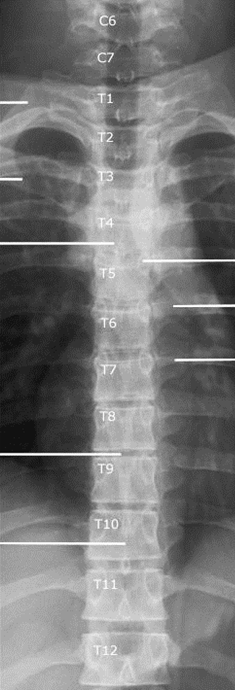
\includegraphics[height=0.3\textheight]{example_vertebrae.png}
	}
	\caption{Пример рентгеновского изображения позвоночника с номерами шейных (C) и грудных (T) позвонков}
	\label{fig:vertebral-column}
\end{figure}

\begin{figure}[ht]
	\centerfloat{
		\hfill
		\subcaptionbox[List-of-Figures entry]{Мягкий снимок}{%
			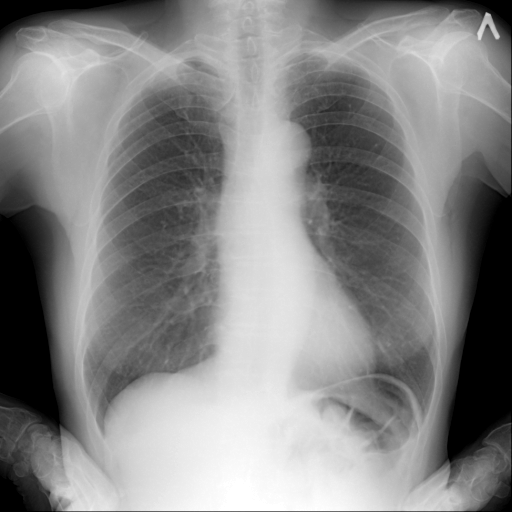
\includegraphics[width=0.3\textwidth]{example_soft.png}}
		\hfill
		\subcaptionbox{Нормальный снимок}{%
			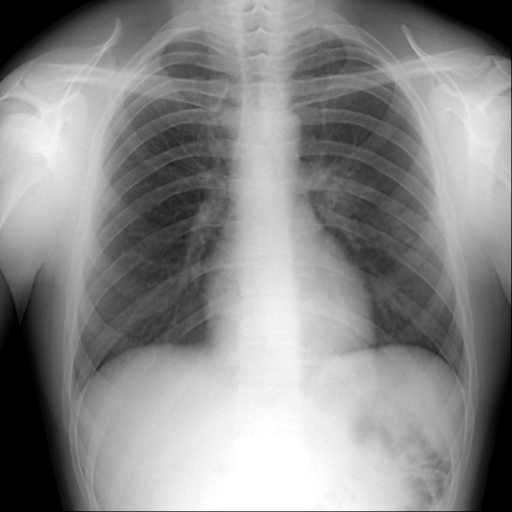
\includegraphics[width=0.3\textwidth]{example_normal.png}}
		\hfill
		\subcaptionbox{Жёсткий снимок}{%
			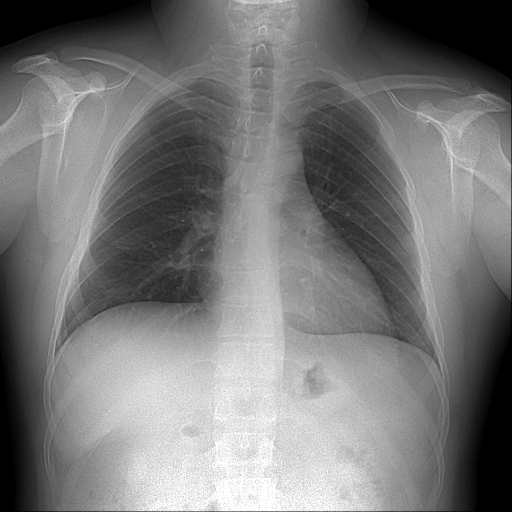
\includegraphics[width=0.3\textwidth]{example_hard.png}}
		\hfill
	}
	\caption{Примеры рентгеновских снимков грудной клетки разной жёсткости}
	\label{fig:samples-different-hardness}
\end{figure}

Настоящее исследование развивает идеи работы \cite{dovganich2022automatic}, где было показано, что оптимизация алгоритма диагностики заболеваний по рентгеновскому снимку грудной клетки для работы с изображениями близкой жёсткости вместе с автоматическим контролем качества рентгеновских изображений позволяет достичь точности классификации выше, чем у алгоритма, созданного в расчёте на обработку разнородных по уровню жёсткости изображений. В ходе выполнения данного исследования был применён полностью нейросетевой подход.

Предлагаемый метод оценки жёсткости включает 2 этапа: обучение и применение. В процессе обучения нейросетевая модель, являющаяся основой метода, однократно настраивается с целью оптимального решения задачи и сохраняется для дальнейшего использования. На этапе применения происходит непосредственный анализ изображений.

Процесс обучения выглядит следующим образом:
\begin{enumerate}[beginpenalty=10000]
	\item предобработка входных данных;
	\item итеративный процесс минимизации функции потерь (функционала, отображающего выходные значения нейросетевой модели в показатель их близости к оптимальным значениям для решения задачи) повторением шагов:
	\begin{enumerate}[beginpenalty=10000]
		\item подача предобработанных выходных данных на вход нейросетевой модели и получение её выходных значений;
		\item получение значения функции потерь для данных выходных значений модели и входных данных;
		\item шаг оптимизации;
		\item замер качества работы алгоритма;
		\item проверка условия ранней остановки процесса минимизации;
	\end{enumerate}
	\item сохранение модели.	
\end{enumerate}

Процесс применения метода состоит из следующих шагов:
\begin{enumerate}[beginpenalty=10000]
	\item предобработка входных данных;
	\item подача предобработанных выходных данных на вход нейросетевой модели и получение её выходных значений.
\end{enumerate}

\subsection{Использованные данные}

При решении рассматриваемой задачи были использованы 2 набора рентгенограмм грудной клетки, снятых во фронтальной проекции.

Первый набор изображений был собран в сотрудничестве с медиками из НПЦ~<<Фтизиатрия>> им. Е.Н.~Андреева в г. Якутск и применялся для обучения нейросетевой модели для метода определения жёсткости рентгенограмм.

Второй набор был сформирован из двух наиболее часто используемых при разработке методов компьютерной диагностики туберкулёза лёгких общедоступных наборов рентгенограмм, ставших, можно сказать, эталонными~\cite{oloko2022systematic, zeyu2022review, singh2022evolution, santosh2022advances}: Montgomery County~\cite{candemir2013lung} и Shenzhen~\cite{jaeger2013automatic}. Так как в большинстве работ наборы Montgomery County и Shenzhen используются вместе~\cite{oloko2022systematic, zeyu2022review}, то было принято решение их объединить и обозначать <<Montgomery"~Shenzhen>> (MC"~SZ). Полученный набор снимков использовался для оценки качества работы разработанного алгоритма на снимках, сделанных в других медицинских учреждениях, на другом оборудовании и при других условиях.

\subsubsection{Набор рентгенограмм грудной клетки SakhaTB} \label{subsubsec:dataset-yak-hardness}

Набор состоит из 1298 рентгеновских снимков грудной клетки больных туберкулёзом лёгких пациентов, собранных в нескольких медицинских учреждениях Республики Саха (Якутия) при помощи стационарных и переносных комплексов оборудования. Разрешение изображений разнится  и находится в диапазоне примерно от 2000x2000 до 3000x3000 пикселей. Большинство рентгенограмм имеет глубину цвета 16 бит, у остальных снимков она равна 8 битам.

Для дальнейшей работы глубина цвета снимков предварительно была приведена к 8 битам, а разрешение путём усреднения соседних пикселей было уменьшено в целое число раз до достижения значений около 1000x1000. Одновременно была проведена нормализация диапазона интенсивности пикселей с отсечением (англ.~clipping) по 0.5\% пикселей с каждого конца гистограммы изображения и обрезкой по 1.5\% пикселей с каждой стороны изображений, чтобы увеличить долю диапазона допустимых значений 8 бит информации, приходящуюся на внутренние органы грудной клетки. Примеры снимков приведены на Рис.~\ref{fig:samples-yak-hardness}.

Подмножество снимков этого набора было выложено вместе с рентгенограммами грудной клетки здоровых пациентов для использования в открытый доступ под названием Sakha"~TB (см.~п.~\ref{sec:sakha-tb}).

\begin{figure}[ht]
	\centerfloat{
    	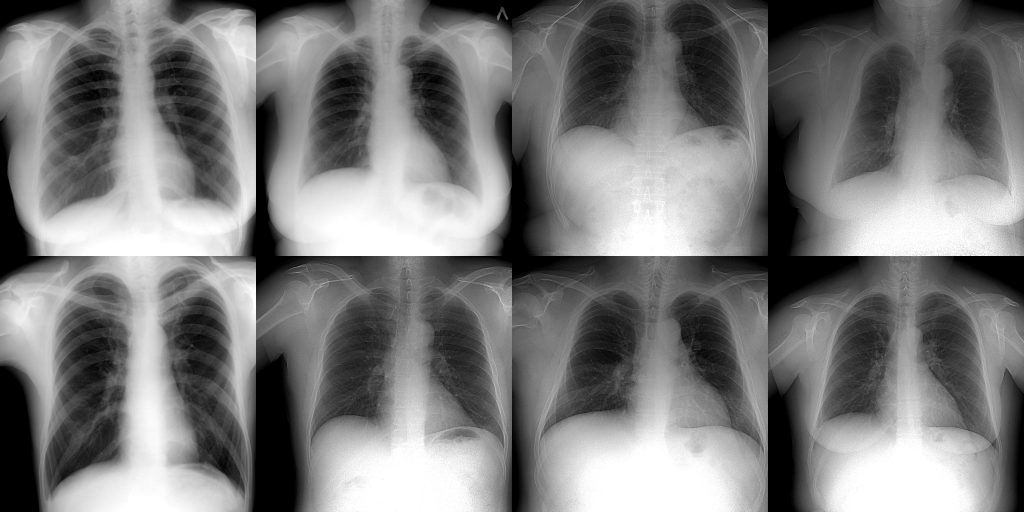
\includegraphics[width=0.9\textwidth]{sakhatb.png}
	}
	\caption{Примеры изображений из набора SakhaTB}
	\label{fig:samples-yak-hardness}
\end{figure}

%\subsubsection{Набор Montgomery County} \label{subsubsec:dataset-mc}

\subsubsection{Набор рентгенограмм грудной клетки Montgomery"~Shenzhen} \label{subsubsec:dataset-mc-sz}

Набор изображений Montgomery County (далее MC) предоставляется Национальной библиотекой медицины Национальных институтов здравоохранения США и собран Министерством здравоохранения и социальных служб США в округе Монтгомери штата Мэриленд. Он содержит рентгеновские снимки грудной клетки в оттенках серого с глубиной цвета 8 бит в формате PNG с разрешением 4020x4892 пикселей и их метки соответствия 2 классам: 80 рентгенограмм здоровых и 58 рентгенограмм больных туберкулёзом лёгких пациентов. %Примеры снимков приведены на Рис.~\ref{fig:samples-mc-sz}.

%\subsubsection{Набор Shenzhen} \label{subsubsec:dataset-sz}

Набор изображений Shenzhen (далее SZ) предоставляется Национальной библиотекой медицины Национальных институтов здравоохранения США и собран Медицинским колледжем провинции Гуандун в Народном госпитале №~3 г.~Шэньчжэнь в КНР. Он содержит рентгеновские снимки грудной клетки в оттенках серого с глубиной цвета 8 бит в формате PNG с различным разрешением (примерно 3000x3000 пикселей) и их метки соответствия 2 классам: 326 рентгенограмм здоровых и 336 рентгенограмм больных туберкулёзом лёгких пациентов.

Примеры снимков объединённого набор приведены на Рис.~\ref{fig:samples-mc-sz}.

%\begin{figure}[ht]
%	\begin{minipage}[b][][b]{0.9\textwidth}\centering
%		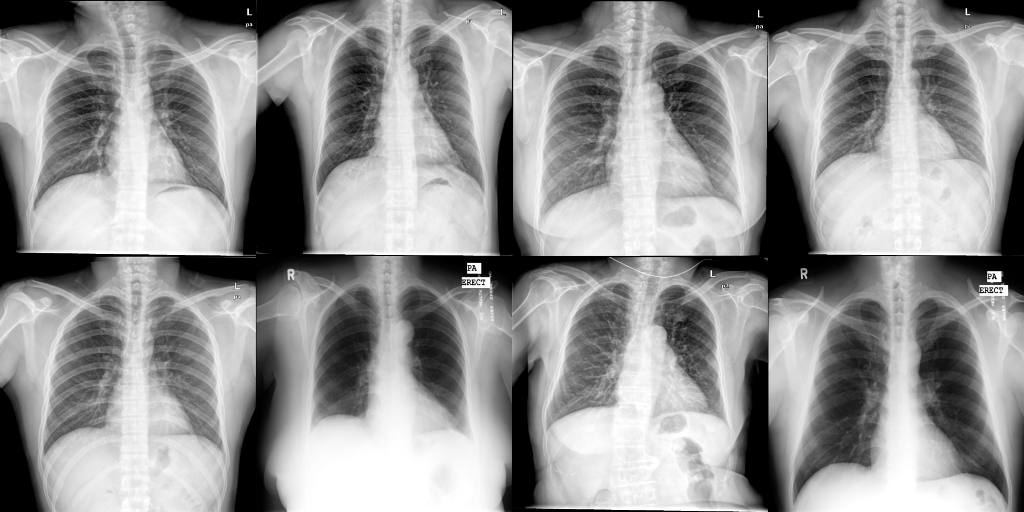
\includegraphics[width=0.9\textwidth]{mcsz-normal.png} \\
%		{а)~Здоровые пациенты}
%	\end{minipage}
%	\hfill
%	\begin{minipage}[b][][b]{0.9\textwidth}\centering
%		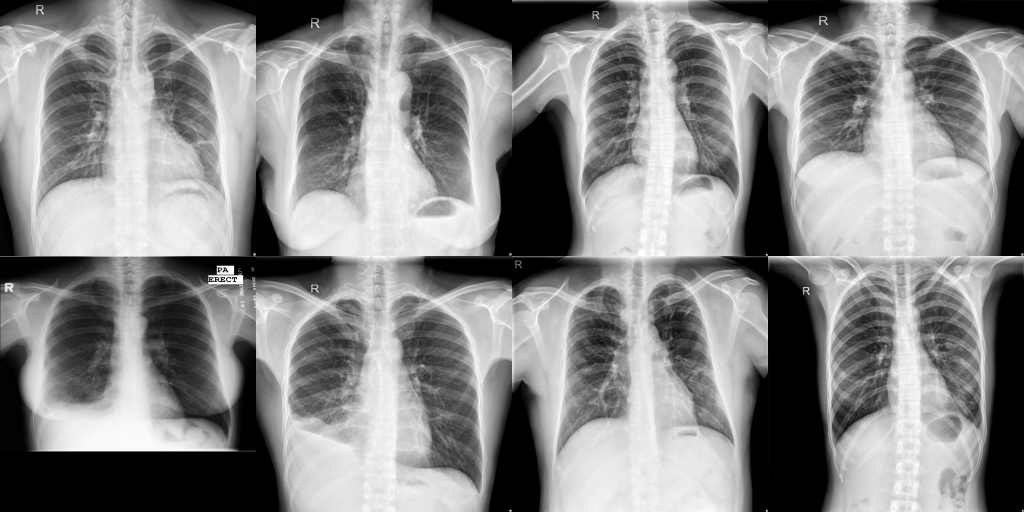
\includegraphics[width=0.9\textwidth]{mcsz-tb.png} \\
%		{б)~Пациенты, больные туберкулёзом}
%	\end{minipage}
%	\caption{Примеры изображений из объединённого набора Montgomery"~Shenzhen (MC"~SZ)}
%	\label{fig:samples-mc-sz}
%\end{figure}

\begin{figure}[ht]
	\centerfloat{
%		\hfill
		\subcaptionbox[List-of-Figures entry]{Здоровые пациенты}{%
			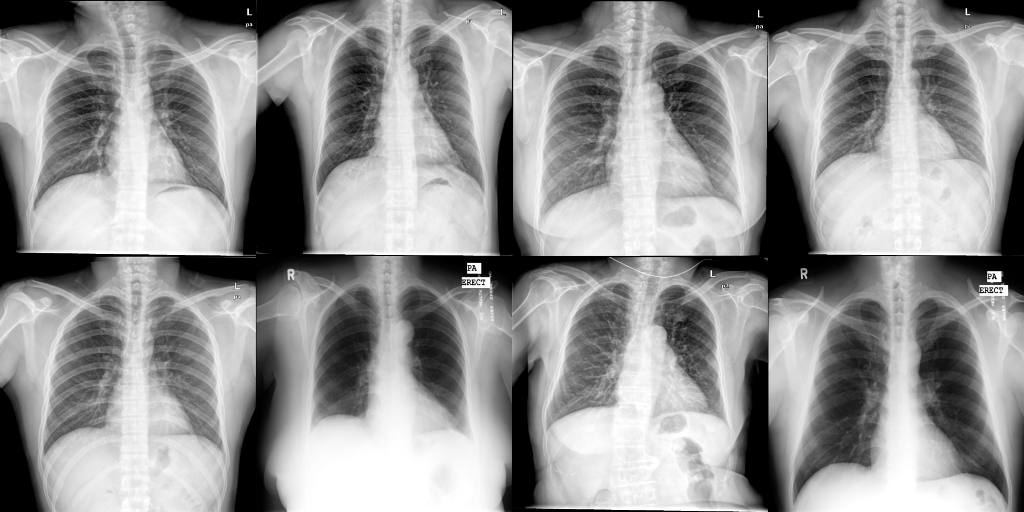
\includegraphics[height=0.25\textheight]{mcsz-normal.png}}
%		\hfill
		\vfill
%		\hfill
		\subcaptionbox{Пациенты, больные туберкулёзом лёгких}{%
			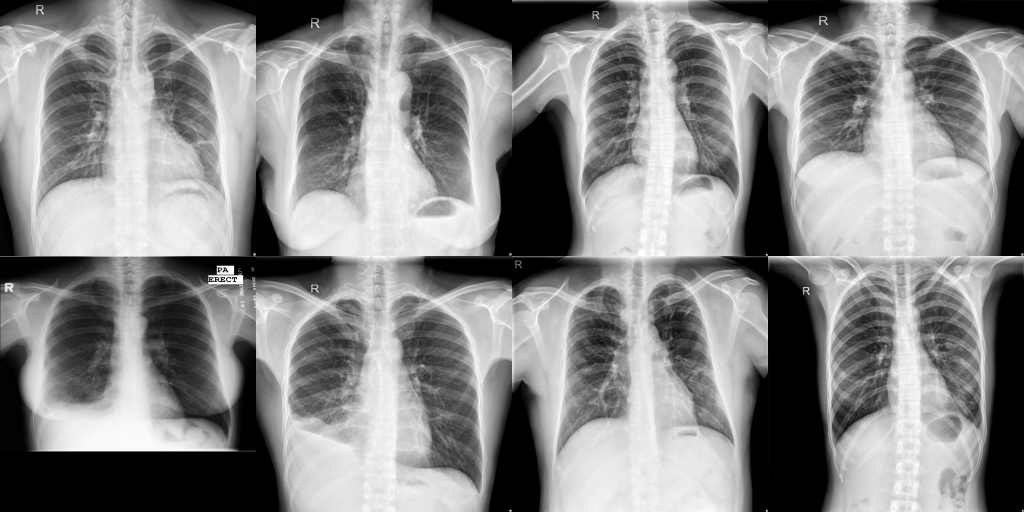
\includegraphics[height=0.25\textheight]{mcsz-tb.png}}
%		\hfill
		\vfill
	}
	\caption{Примеры изображений из объединённого набора Montgomery"~Shenzhen (MC"~SZ)}
	\label{fig:samples-mc-sz}
\end{figure}

\subsubsection{Аннотирование данных}

Для обоих наборов (SakhaTB, собранный в рамках исследования, и MC"~SZ) была проведена процедура аннотации врачом-рентгенологом из НПЦ~<<Фтизиатрия>> им. Е.Н.~Андреева в г. Якутск. В рамках процедуры каждому изображению ставился в соответствие его уровень жёсткости, выраженный числом отчётливо видимых на этом снимке верхних грудных позвонков.  Распределение изображений по такому показателю жёсткости представлено на Рис.~\ref{fig:vertebrae-yak-hardness}"~\ref{fig:vertebrae-mc-sz}.

\begin{figure}[ht]
	\centerfloat{
		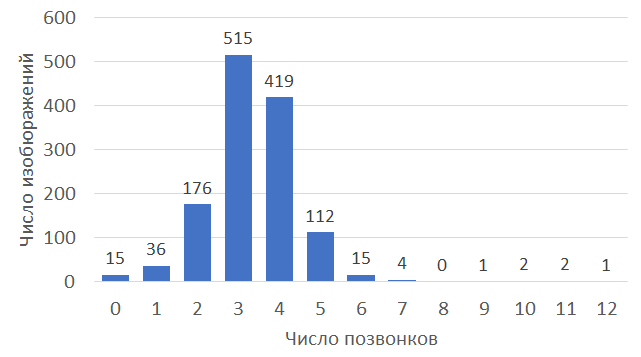
\includegraphics[height=0.3\textheight]{total_vertebrae_hist.png}
	}
	\caption{Гистограмма распределения снимков набора SakhaTB по числу отчётливо видимых позвонков}
	\label{fig:vertebrae-yak-hardness}
\end{figure}

\begin{figure}[ht]
	\centerfloat{
		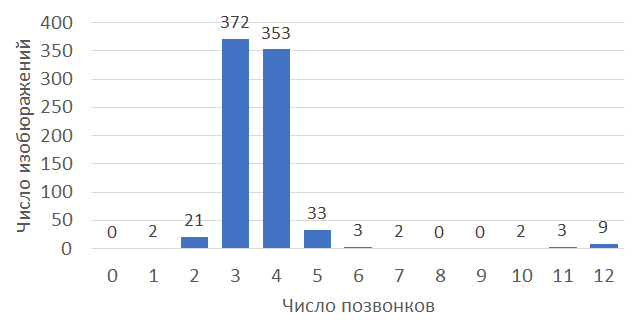
\includegraphics[height=0.25\textheight]{total_vertebrae_hist_mc-sz.png}
	}
	\caption{Гистограмма распределения снимков набора MC"~SZ по числу отчётливо видимых позвонков}
	\label{fig:vertebrae-mc-sz}
\end{figure}

\subsection{Адаптивная предобработка входных изображений} \label{subsec:tb-hardness-preprocessing}

Хотя финальным критерием при определении уровня жёсткости рентгеновского снимка грудной клетки является число чётко контурируемых верхних грудных позвонков~\cite{тимофеева2013основные, сидоров2012методика}, для определения уровня контраста перед исследованием требуется обращать внимание на видимость других областей грудной клетки, (например, на элементы лёгочного рисунка) и органов~\cite{сидоров2012методика}. На основании этого было принято решение не ограничивать область исследования на снимках пределами грудной клетки, а рассматривать изображения целиком.

Так как условия получения снимка, характеристики тела пациента и принципы считывания сигнала и хранения информации каждого конкретного устройства могут сильно влиять на характер рентгеновских изображений, перед подачей их на вход алгоритму определения жёсткости выполнялся этап предобработки, который заключается в последовательности следующих шагов:
\begin{enumerate}[beginpenalty=10000]
	\item автоматическое контрастирование изображения:
	\begin{equation}
	h \left( x \right) = 255 \cdot \frac{x - p_{0.5}}{p_{99.5} - p_{0.5}}, \nonumber
	\end{equation}
	где $x$ "--- значение интенсивности пикселя входного изображения, $p_{0.5}$ и $p_{99.5}$ "--- это 0.5\%"~ и 99.5\%"~процентили значений интенсивности всех пикселей изображения;
	\item автоматическая гамма-коррекция интенсивности пикселей изображения:
	\begin{equation}
	g \left( x \right) = 255 \cdot {\left( \frac{x}{255} \right)}^{\gamma}, \quad \gamma = \log_{\mu / 255}{0.5}, \nonumber
	\end{equation}
	где $\mu$ "--- средняя интенсивность всего изображения;
	\item уменьшение изображения до входного разрешения, используемого нейронной сетью (512х512 пикселей для модели ResNet"~18 и 384x384 пикселей для EfficientNetV2"~S).
	\item опциональный шаг глобальной или локальной (CLAHE~\cite{pizer1987adaptive}) эквализации гистограммы. Размер стороны квадратного окна  в пикселях, используемого в методе локальной эквализации гистограммы, прямо зависит от размера стороны изображения и составляет $\frac{1}{2^n}$ от него, где $n\in\mathbb{N}$ "--- параметр метода. Влияние наличия этого шага и размера окна на качество работы алгоритма будет показано ниже.
\end{enumerate}

\subsection{Метод определения жёсткости рентгеновских снимков грудной клетки}

Так как уровень жёсткости рентгеновского снимка "--- это упорядоченная величина, для сохранения отношений упорядоченности между классами задача его определения рассматривалась как задача порядковой регрессии (также иногда называется порядковой классификацией)~\cite{7161338, 353a0d24-9c24-3a11-a330-afc86b9c39c8}.

Для решения задачи автоматического определения жёсткости рентгеновского снимка грудной клетки был разработан нейросетевой метод. На вход алгоритма поступает рентгеновский снимок грудной клетки и подвергается предобработке, затем при помощи нейронной сети ему ставится в соответствие вещественное число на отрезке $\left[0, 1\right]$, которое является внутренним безразмерным показателем жёсткости снимка, на основании которого после сравнения с настраиваемыми порогами изображение относится к одному из рассматриваемых классов жёсткости.  Пороги являются частью модели и настраиваются вместе с весами слоёв нейронной сети в процессе обучения. Преимуществом такого подхода является то, что с помощью внутреннего показателя жёсткости можно ранжировать изображения относительно друг друга даже в том случае, когда обрабатываемое изображение значительно отличается от обучающей выборки и для такого снимка пороги разделения классов жёсткости могут быть настроены неверно.

Для решения задач обработки медицинских изображений и, в частности, диагностики заболеваний широко используются~\cite{oloko2022systematic} свёрточные нейронные сети семейств ResNet~\cite{he2016deep}, DenseNet~\cite{huang2017densely} и др.

В ходе исследования для решения задачи определения жёсткости снимков, вследствие малого размера выборки, была использована компактная сеть ResNet"~18 с меньшим числом параметров и, следовательно, меньшей склонностью к переобучению по сравнению с более крупными сетями этой же архитектуры или представителями других вышеупомянутых архитектур.

Также было проведено сравнение качества решения этой задачи с таковым у компактной сети более новой архитектуры свёрточных нейронных сетей EfficientNetV2"~S~\cite{tan2021efficientnetv2}, так как в задачах классификации изображений она проявляет себя лучше перечисленных выше. Её основное отличие от них заключается в оптимизации работы свёрточных слоёв с помощью их пропорционального масштабирования, смены порядка операций разной размерности, уменьшения размера ядер свёртки и отказа от «тяжёлых» слоёв, что позволяет уменьшить потребление памяти и задействовать освободившиеся ресурсы на увеличение глубины и обобщающей способности нейронной сети.

\subsection{Эксперименты и результаты} \label{subsec:tb-hardness-experiments}

Как видно из Рис.~\ref{fig:vertebrae-yak-hardness}, набор изображений значительно несбалансирован и для ряда подуровней жёсткости содержит крайне мало примеров. Исходя из этого было принято решение, используя определённое врачом-рентгенологом число отчётливо видимых на снимках верхних грудных позвонков, разделить все снимки по уровню жёсткости на 3 группы, ориентируясь на медицинские критерии: мягкие (видно менее 3 позвонков), нормальные (видно 3"~4 позвонка) и жёсткие (видно более 4 позвонков)~\cite{тимофеева2013основные, сидоров2012методика}. Количество снимков в сформированных группах представлено на Рис.~\ref{fig:hardness-yak-hardness}. Именно эти три класса рассматривались в качестве допустимых значений целевой переменной для задачи порядковой регрессии.

\begin{figure}[ht]
	\centerfloat{
		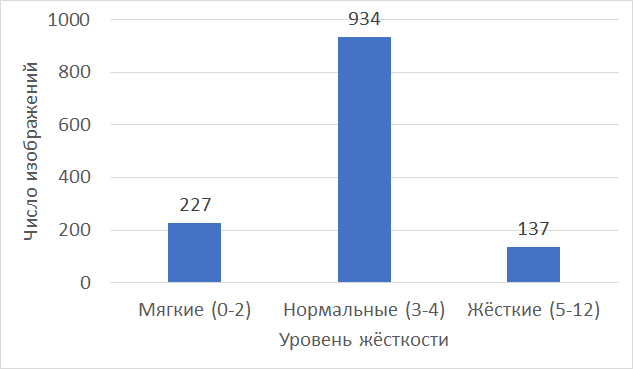
\includegraphics[height=0.25\textheight]{total_hardness_hist.png}
	}
	\caption{Гистограмма распределения снимков набора SakhaTB по уровню жёсткости}
	\label{fig:hardness-yak-hardness}
\end{figure}

Для ускорения процесса обучения за счёт наличия готовых низкоуровневых фильтров при решении обеих задач в качестве начального состояния нейронной сети использовались веса соответствующей модели, обученной на решение задачи классификации изображений реального мира ImageNet"~1K~\cite{russakovsky2015imagenet}. Последний слой был заменён на полносвязный слой с 1 выходом и 2 настраиваемыми в процессе обучения параметрами"=порогами пороговой модели порядковой регрессии~\cite{rennie2005loss}, во время дальнейшего обучения были задействованы все слои.

Все базовые наборы изображений и их рассмотренные комбинации делились на обучающую, валидационную и тестовую выборки в соотношении 64:16:20 с предварительным случайным перемешиванием изображений и стратификацией по классу жёсткости для сохранения пропорций между классами. Изображения обучающей выборки в процессе обучения последовательно подвергались четырём случайным преобразованиям, а именно:
\begin{enumerate}[beginpenalty=10000]
	\item поворотам (в пределах 15 градусов в каждую сторону),
	\item масштабированию (коэффициент выбирался случайно из отрезка $\left[ 0.8, 1.2 \right]$,
	\item сдвигам (до 30\% размера изображения по каждой оси),
	\item изменению яркости и контраста (до 20\% в каждую сторону).
\end{enumerate}

В качестве функции потерь в процессе обучения и валидации была выбрана функция потерь пороговой порядковой регрессии в виде суммы слагаемых, число которых зависит от числа классов (all"=threshold)~\cite{rennie2005loss}:

\begin{equation}
	\begin{cases}
		L \left( z, y \right) = \sum_{k=1}^{K-1} f \left( s \left( k, y \right) \cdot \left( \theta_k-z \right) \right), \\
		s \left( k, y \right) =
		\begin{cases}
			-1, k < y, \\
			+1, \ k \geq y,
		\end{cases}
	\end{cases} \nonumber
\end{equation}

\noindent где $z$ "--- выход нейронной сети (безразмерный показатель жёсткости), принимающий значения из отрезка $\left[ 0, 1 \right]$ (чем ближе к $1$, тем выше жёсткость снимка), $y$ "--- истинный класс соответствующего этому выходу изображения, $K$ "--- общее число классов, $\theta_1 < \theta_2 < \ldots < \theta_{K-1}$ "--- пороги, делящие действительную прямую на $K$ частей, а $f(x)$ "--- базовая функция потерь бинарной классификации, в качестве которой использовалась логистическая функция потерь:

\begin{equation}
	f \left( x \right) = \ln{\frac{1}{1+e^{-x}}}. \nonumber
\end{equation}

Так как даже после сведения количества классов в задаче порядковой регрессии к трём выборка всё равно осталась сильно несбалансированной, то применялось взвешивание значений функции потерь для каждого примера с весами, обратно пропорциональными количеству изображений соответствующего класса. В роли показателя качества порядковой регрессии на этапе валидации выступала сбалансированная по классам средняя абсолютная ошибка (macro"=averaged MAE, далее mMAE)~\cite{baccianella2009evaluation}.

Также в целях получения базовой оценки качества решения задачи была обучена модель для обыкновенной классификации изображений на 3 класса. Последний слой модели"=основы был заменён на полносвязный с 3 выходами. Роль функции потерь выполняла кросс-энтропия:

\begin{equation}
	\begin{cases}
		CE \left( z,y \right) = \sum_{k=1}^{K}{\mathbb{I} \left[ y = k \right] \cdot \ln{\left( softmax \left( z \right)_k \right)}}, \\
		softmax \left( z \right)_k = \frac{e^{z_k}}{\sum_{i=1}^{K}e^{z_i}},\quad \mathbb{I} \left[ y = k \right] =
		\begin{cases}
			1, y = k, \\
			0, y \neq k,
		\end{cases}
	\end{cases} \nonumber
\end{equation}

\noindent а роль показателя качества на этапе валидации "--- сбалансированная точность (далее BalAcc)~\cite{brodersen2010balanced}.

Для оптимизации функции потерь применялся алгоритм градиентного спуска AdamW~\cite{loshchilov2018decoupled} с параметрами $lr = 5 \cdot {10}^{-6}$, $\beta_1 = 0.9$, $\beta_2 = 0.999$, $\lambda = 0.01$. Размер пакета (англ.~batch) изображений был равен 64 для модели на основе ResNet"~18 и 16 для модели на основе EfficientNetV2"~S; в обоих случаях применялось накопление градиента на протяжении 8 и 2 итераций соответственно (до достижения размера <<виртуального пакета>> в 128 объектов). В конце каждой эпохи качество модели замерялось на валидационной выборке; при отсутствии уменьшения значения функции потерь на ней в течение 10 эпох шаг градиентного спуска уменьшался в 5 раз, а при отсутствии улучшения в течение 31 эпохи обучение прекращалось. Переобучение контролировалось замерами функции потерь и вышеуказанных показателей качества, однако значительного ухудшения качества работы модели на валидационной выборке с течением времени не наблюдалось (см.~Рис.~\ref{fig:val-losses}; можно заметить небольшой рост значений функции потерь у модели на основе EfficientNetV2"~S, что свидетельствует о некотором переобучении модели), поэтому в качестве финального состояния принималось значение весов модели в конце последней эпохи.

\begin{figure}[ht]
	\centerfloat{
		\hfill
		\subcaptionbox[List-of-Figures entry]{ResNet"~18}{%
			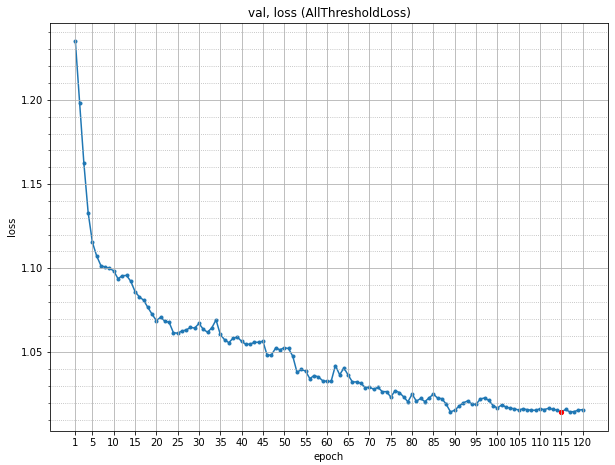
\includegraphics[width=0.48\textwidth]{val_loss_ord-clahe2.png}}
		\hfill
		\subcaptionbox{EfficientNetV2"~S}{%
			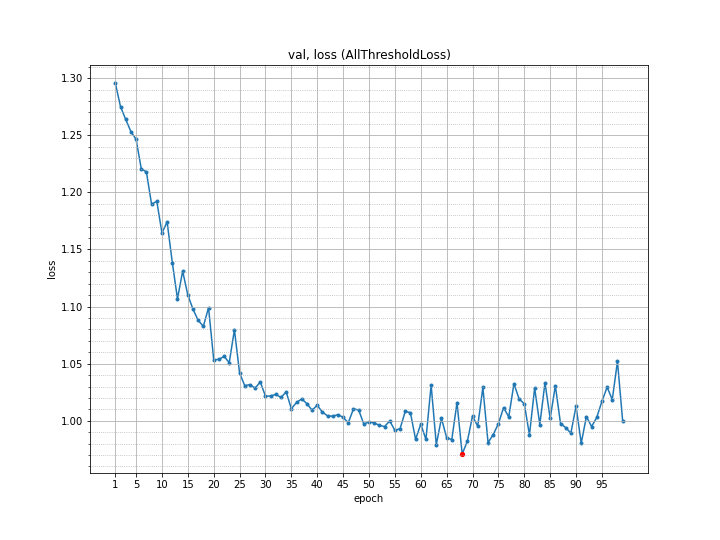
\includegraphics[width=0.48\textwidth]{val_loss_eff.png}}
		\hfill
	}
	\caption{Примеры графиков зависимости функции потерь от количества эпох на валидационной выборке в задаче анализа жёсткости снимков грудной клетки}
	\label{fig:val-losses}
\end{figure}

Итоговые значения показателей качества, полученные на тестовой выборке, представлены в Табл.~\ref{tab:hardness-metrics-test}. Модели для решения задачи порядковой регрессии содержат «ord» в своём названии, модель для решения задачи классификации "--- <<clf>>. Модель <<ord"~eff>>, была создана на основе EfficientNetV2"~S, а остальные модели "--- на основе ResNet"~18. В столбце <<Эквализация гистограммы>> стоит прочерк, если эквализация не применялась; <<глобальная>> в случае использования глобальной эквализации; размер окна локальной эквализации гистограммы в виде доли от размера всего изображения в случае использования локальной эквализации.

На основании сбалансированной точности и сбалансированной MAE лучшей моделью оказалась модель порядковой регрессии с локальной эквализацией гистограммы на этапе предобработки снимков с окном, длина стороны которого была равна $\frac{1}{2}$ длины стороны изображения. Далее для краткости она будет обозначена <<ord"~clahe2>>. Дальнейший анализ изображений проводится с использованием этой модели.

\begin{table} [htbp]%
	\centering
	\caption{Значения показателей качества работы алгоритмов определения жёсткости на тестовой выборке набора SakhaTB}%
	\label{tab:hardness-metrics-test}% label всегда желательно идти после caption
	\renewcommand{\arraystretch}{1.5}%% Увеличение расстояния между рядами, для улучшения восприятия.
	\begin{SingleSpace}
		\begin{tabular}{@{}@{\extracolsep{20pt}}lccc@{}} %Вертикальные полосы не используются принципиально, как и лишние горизонтальные (допускается по ГОСТ 2.105 пункт 4.4.5) % @{} позволяет прижиматься к краям
			\toprule     %%% верхняя линейка
			Модель & Эквализация гистограммы & BalAcc & mMAE \\
			\midrule %%% тонкий разделитель. Отделяет названия столбцов. Обязателен по ГОСТ 2.105 пункт 4.4.5
			clf	& - & 0.563 & 0.452 \\
			ord"~eff & - & 0.623 & 0.399 \\
			ord & - & 0.609 & 0.452 \\
			ord"~glob & глобальная & 0.609 & 0.452 \\
			\textbf{ord"~clahe2} & \textbf{$\frac{1}{2}$ стороны изображения} & \textbf{0.636} & \textbf{0.398} \\
			ord"~clahe4 & $\frac{1}{4}$ стороны изображения	& 0.610 & 0.449 \\
			ord"~clahe8 & $\frac{1}{8}$ стороны изображения	& 0.593 & 0.468 \\
			ord"~clahe16 & $\frac{1}{16}$ стороны изображения & 0.600 & 0.468 \\
			\bottomrule %%% нижняя линейка
		\end{tabular}%
	\end{SingleSpace}
\end{table}

На Рис.~\ref{fig:hardness-class-separation} представлена зависимость вероятностей классов <<Жёсткий>>~(Hard) и <<Мягкий>>~(Soft), предсказанных моделью <<clf>> для решения задачи простой классификации, а также безразмерной величины жёсткости, предсказанной моделью <<ord"~clahe2>> для задачи порядковой регрессии, и истинного значения уровня жёсткости объектов тестовой выборки. Можно заметить, что разделение классов далеко от идеального.

\begin{figure}[ht]
	\centerfloat{
		\hfill
		\subcaptionbox[List-of-Figures entry]{<<clf>> (простая классификация)}{%
			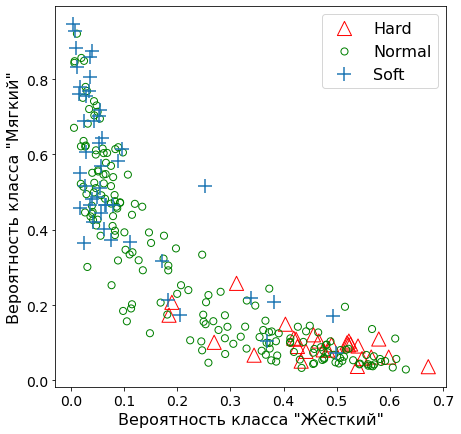
\includegraphics[width=0.45\textwidth]{clf_separation.png}}
		\hfill
		\subcaptionbox{<<ord"~clahe2>> (порядковая регрессия)}{%
			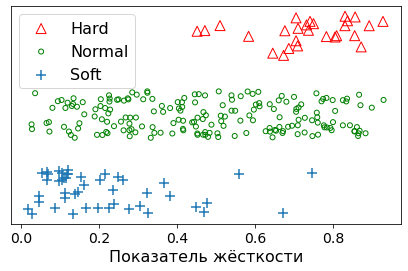
\includegraphics[width=0.45\textwidth]{ord_separation.png}}
		\hfill
	}
	\caption{Зависимость предсказаний моделей в зависимости от истинного класса объекта для набора SakhaTB}
	\label{fig:hardness-class-separation}
\end{figure}

Как выяснилось после проверки ошибочно классифицированных снимков, причиной тому послужила шумность использованного набора данных из-за неоднозначности и недостаточной определённости критериев разметки. Подтверждением этого предположения также служит близость значений меры качества на обучающей выборке к таковым на тестовой выборке: сбалансированная точность около 0.70 и 0.67 у моделей <<clf>> и <<ord"~clahe2>> соответственно.

Рассмотрение задачи определения жёсткости рентгеновского снимка как задачи порядковой регрессии позволяет, используя полученную для её решения модель, с некоторой точностью ранжировать изображения по жёсткости на основе внутреннего показателя жёсткости нейронной сети. В качестве меры качества ранжирования был выбран коэффициент ранговой корреляции Спирмена~\cite{zwillinger1999crc}, так как он позволяет обнаруживать в том числе нелинейные зависимости рассматриваемых величин. Замеры делались относительно указанных врачом количества чётко видимых на снимке позвонков и относительно классов жёсткости снимков. Полученные значения приведены в Табл.~\ref{tab:hardness-spearman-test}.

\begin{table} [htbp]%
	\centering
	\caption{Значения показателя качества ранжирования тестовой выборки набора SakhaTB алгоритмом определения жёсткости}%
	\label{tab:hardness-spearman-test}% label всегда желательно идти после caption
	\renewcommand{\arraystretch}{1.5}%% Увеличение расстояния между рядами, для улучшения восприятия.
	\begin{SingleSpace}
		\begin{tabular}{@{}@{\extracolsep{20pt}}lcc@{}} %Вертикальные полосы не используются принципиально, как и лишние горизонтальные (допускается по ГОСТ 2.105 пункт 4.4.5) % @{} позволяет прижиматься к краям
			\toprule     %%% верхняя линейка
			Модель & Spearman (позвонки) & Spearman (жёсткость) \\
			\midrule %%% тонкий разделитель. Отделяет названия столбцов. Обязателен по ГОСТ 2.105 пункт 4.4.5
			ord"~eff & 0.564 & 0.457 \\
			ord & 0.576 & 0.497 \\
			ord"~glob & 0.599 & 0.514 \\
			\textbf{ord"~clahe2} & \textbf{0.606} & \textbf{0.534} \\
			ord"~clahe4 & 0.602 & 0.519 \\
			ord"~clahe8 & 0.588 & 0.498 \\
			ord"~clahe16 & 0.596 & 0.507 \\
			\bottomrule %%% нижняя линейка
		\end{tabular}%
	\end{SingleSpace}
\end{table}

Была проведена оценка качества работы модели <<ord"~clahe2>> на наборе MC"~SZ. Результаты сравнения качества работы алгоритма на наборе MC"~SZ и на тестовой выборке набора SakhaTB приведены в Табл.~\ref{tab:hardness-metrics-mc-sz}.

\begin{table} [htbp]%
	\centering
	\caption{Значения показателя качества ранжирования тестовой выборки набора SakhaTB алгоритмом определения жёсткости}%
	\label{tab:hardness-metrics-mc-sz}% label всегда желательно идти после caption
	\renewcommand{\arraystretch}{1.5}%% Увеличение расстояния между рядами, для улучшения восприятия.
	\begin{SingleSpace}
		\begin{tabulary}{0.9\textwidth}{@{}@{\extracolsep{20pt}}lCCCC@{}} %Вертикальные полосы не используются принципиально, как и лишние горизонтальные (допускается по ГОСТ 2.105 пункт 4.4.5) % @{} позволяет прижиматься к краям
			\toprule     %%% верхняя линейка
			Набор данных & BalAcc & mMAE & Spearman \mbox{(позвонки)} & Spearman \mbox{(жёсткость)} \\
			\midrule %%% тонкий разделитель. Отделяет названия столбцов. Обязателен по ГОСТ 2.105 пункт 4.4.5
			Набор SakhaTB & 0.636 & 0.398 & 0.606 & 0.534 \\
			MC"~SZ & 0.546 & 0.565 & 0.325 & 0.203 \\
			\bottomrule %%% нижняя линейка
		\end{tabulary}%
	\end{SingleSpace}
\end{table}

\section{Использование результатов оценки качества рентгеновских снимков при нейросетевой диагностике туберкулёза лёгких}

Результаты оценки жёсткости рентгенограмм могут быть использованы, например, для предварительной фильтрации обучающей выборки и входных данных нейросетевого алгоритма компьютерной диагностики туберкулёза лёгких. Как показано в работе~\cite{dovganich2022automatic}, такая фильтрация, а также создание отдельных моделей для разных уровней жёсткости снимков позволяют повысить робастность и точность метода компьютерной диагностики. В этом разделе демонстрируется влияние предварительной фильтрации обучающей и валидационной выборок на качество работы алгоритма классификации в задаче диагностики туберкулёза лёгких по рентгеновским снимкам грудной клетки.

\subsection{Формирование набора данных} \label{subsubsec:dataset-tbx}

Так как в экспериментах этапу обучения модели в задаче диагностики туберкулёза лёгких предшествует этап фильтрации снимков на основании уровня жёсткости, то в целях поддержания размера обучающей и валидационной выборок после прореживания на достаточном уровне, а также для создания более разнородных выборок, как и в работе ~\cite{dovganich2022automatic}, для создания нейросетевого метода диагностики и замера влияния фильтрации на качество диагностики использовался набор рентгенограмм, состоящий из двух частей: уже упомянутый в п.~\ref{subsubsec:dataset-mc-sz} составной набор MC"~SZ и ещё один из часто применяемых при разработке методов компьютерной диагностики туберкулёза лёгких общедоступных наборов рентгенограмм~\cite{singh2022evolution, santosh2022advances} "--- TBX11K~\cite{liu2020rethinking}.

%\subsubsection{Набор TBX11K} \label{subsubsec:dataset-tbx} % перенёс метку в родительскую \subsection

Набор TBX11K подготовлен в Нанькайском университете г.~Тяньцзин в КНР. Он состоит из 11200 рентгеновских снимков грудной клетки в оттенках серого с глубиной цвета 8 бит в формате PNG с разрешением 512x512 пикселей. Он изначально поделён на обучающую, валидационную и тестовую выборки, при этом последняя не имеет разметки, поэтому из всего набора только для 8400 изображений доступны метки принадлежности к одному из 3 классов (3800 здоровых и 800 больных туберкулёзом лёгких пациентов, а также больные иными заболеваниями пациенты) и границы поражённых областей лёгких. В рамках исследования использовались только снимки здоровых и больных туберкулёзом лёгких пациентов, а остальные были исключены из рассмотрения. Примеры изображений из набора представлены на Рис.~\ref{fig:samples-tbx}.

\begin{figure}[ht]
	\centerfloat{
%		\hfill
		\subcaptionbox[List-of-Figures entry]{Здоровые пациенты}{%
			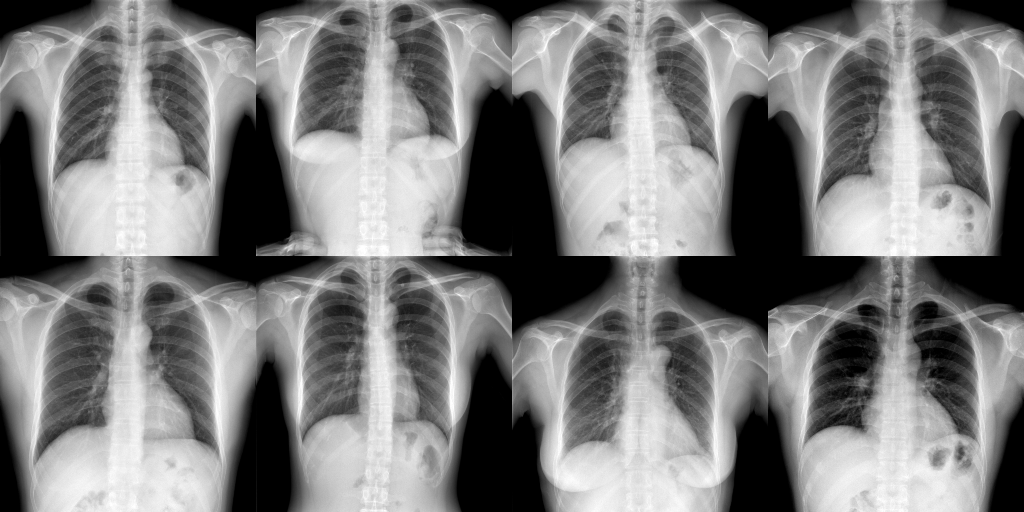
\includegraphics[height=0.25\textheight]{tbx11k_normal.png}}
%		\hfill
		\vfill
%		\hfill
		\subcaptionbox{Пациенты, больные туберкулёзом лёгких}{%
			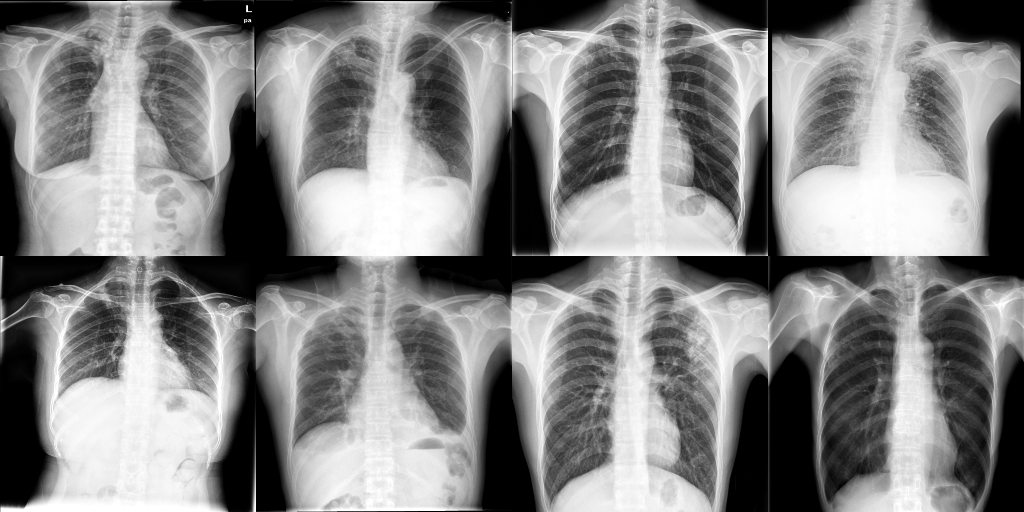
\includegraphics[height=0.25\textheight]{tbx11k_tb.png}}
%		\hfill
		\vfill
	}
	\caption{Примеры изображений из набора TBX11K}
	\label{fig:samples-tbx}
\end{figure}

Рентгенограммам здоровых пациентов из получившегося объединённого набора были поставлены в соответствие метки класса NORMAL, а больных туберкулёзом лёгких пациентов "--- класса TB. Итоговое число снимков каждого класса в объединённом наборе, а также в его отдельных частях приведено в Табл.~\ref{tab:hardness-dataset-size}.

\begin{table} [htbp]%
	\centering
	\caption{Размеры использованных наборов данных}%
	\label{tab:hardness-dataset-size}% label всегда желательно идти после caption
	\renewcommand{\arraystretch}{1.5}%% Увеличение расстояния между рядами, для улучшения восприятия.
	\begin{SingleSpace}
		\begin{tabulary}{\textwidth}{@{}@{\extracolsep{10pt}}lCCC@{}} %Вертикальные полосы не используются принципиально, как и лишние горизонтальные (допускается по ГОСТ 2.105 пункт 4.4.5) % @{} позволяет прижиматься к краям
			\toprule     %%% верхняя линейка
			Название набора & Число снимков класса NORMAL & Число снимков класса TB & Общее число снимков \\
			\midrule %%% тонкий разделитель. Отделяет названия столбцов. Обязателен по ГОСТ 2.105 пункт 4.4.5
			Montgomery & 80 & 58 & 138 \\
			Shenzhen & 326 & 336 & 662 \\
			TBX11K & 3800 & 800 & 4600 \\
			\midrule
			Всего & 4206 & 1194 & 5400 \\
			\bottomrule %%% нижняя линейка
		\end{tabulary}%
	\end{SingleSpace}
\end{table}

\subsection{Метод компьютерной диагностики туберкулёза лёгких}\label{subsec:tbx-diagnostics}

Использованный в этом разделе для экспериментов алгоритм диагностики туберкулёза лёгких выглядел следующим образом:
\begin{enumerate}[beginpenalty=10000]
	\item поступивший на вход рентгеновский снимок грудной клетки подвергается предобработке, совпадающей с описанной в п.~\ref{subsec:tb-hardness-preprocessing} за исключением того, что эквализация гистограммы не проводилась;
	\item при помощи нейросетевой модели ему ставятся в соответствие 2 вещественных числа из отрезка $\left[ 0, 1 \right]$, которые выражают предсказанные веса классов NORMAL и TB (сумма весов для каждого изображения равна 1);
	\item класс, чей вес больше, принимается за выходное значение алгоритма.
\end{enumerate}

В качестве основы для нейросетевой модели использовалась сеть EfficientNetV2"~S, последний слой которой был заменён на полносвязный слой с 2 выходами. Процедуры деления набора данных на подвыборки и обучения модели со взвешиванием классов для балансировки, а также начальные состояния весов сети совпадали с описанными в п.~\ref{subsec:tb-hardness-experiments}. В роли функции потерь выступала кросс"=энтропия, а в роли меры качества "--- сбалансированная точность.

%В качестве основ для нейронных сетей использовались EfficientNetV2"~S и ResNet"~18, последний слой которых заменялся на полносвязный с 2 выходами. Процедуры деления набора данных на подвыборки и обучения модели со взвешиванием классов для балансировки, а также начальные состояния весов и этапы предобработки были аналогичны таковым из метода в предыдущем разделе, однако эквализация гистограммы не проводилась. В роли функции потерь выступала кросс"=энтропия, а в роли меры качества "--- сбалансированная точность.
%
%При решении этой задачи из двух моделей лучшее качество классификации до прореживания показала модель на основе EfficientNetV2"~S, и именно она участвует в сравнении. Вероятно, это обусловлено значительно возросшим объёмом и качеством выборки. 

\subsection{Эксперименты и результаты}

Рентгенограммы из наборов MC"~SZ и TBX11K были обработаны разработанным алгоритмом оценки жёсткости. Распределение снимков из тестовой выборки сформированного в п.~\ref{subsubsec:dataset-yak-hardness} набора и из этих двух наборов по безразмерному показателю жёсткости, предсказанному моделью <<ord"~clahe2>>, представлен на Рис.~\ref{fig:ordinal-hist-total}. Однако следует осторожно относиться к разделению снимков из наборов MS"~SZ и TBX11K на классы жёсткости, так как истинные пороги разделения классов для этих данных могут сильно отличаться от полученных моделью на этапе обучения в п.~\ref{subsec:tb-hardness-experiments} из-за их визуального отличия от изображений её обучающей выборки.

\begin{figure}[ht]
	\centerfloat{
		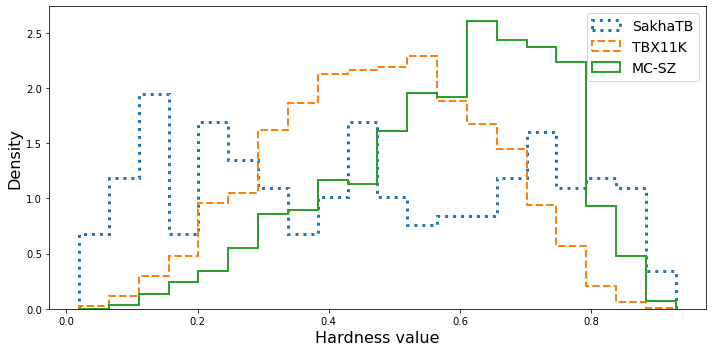
\includegraphics[height=0.3\textheight]{total_ordinal_hist_eng.png}
	}
	\caption{Гистограммы распределения снимков трёх использованных наборов изображений по предсказанному моделью <<ord"~clahe2>> показателю жёсткости}
	\label{fig:ordinal-hist-total}
\end{figure}

Отдельные гистограммы для классов NORMAL и TB для наборов MC"~SZ и TBX11K представлены на Рис.~\ref{fig:ordinal-hist-datasetwise}. Небольшие различия гистограмм классов совпадают с визуальной разницей между снимками этих классов: класс TB в обоих из них содержит больше мягких снимков, а классы NORMAL "--- больше жёстких (см.~Рис.~\ref{fig:samples-mc-sz}~и~\ref{fig:samples-tbx}).

\begin{figure}[ht]
	\centerfloat{
		\subcaptionbox[List-of-Figures entry]{MC"~SZ}{%
			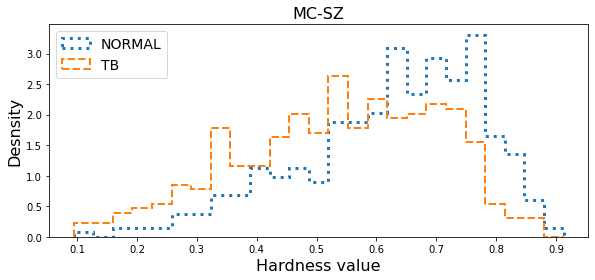
\includegraphics[height=0.25\textheight]{mcsz_ordinal_hist_eng_1.png}}
		
		\subcaptionbox{TBX11K}{%
			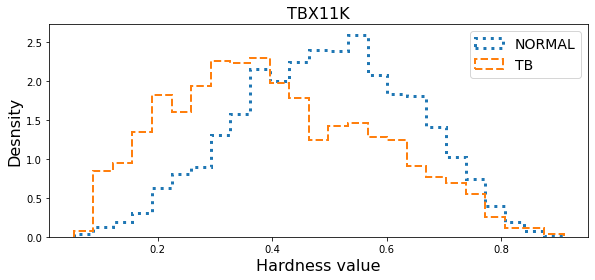
\includegraphics[height=0.25\textheight]{tbx11k_ordinal_hist_eng_1.png}}
	}
	\caption{Гистограммы распределения снимков каждого класса для использованных в задаче диагностики туберкулёза лёгких наборов изображений MC"~SZ и TBX11K по предсказанному моделью <<ord"~clahe2>> показателю жёсткости}
	\label{fig:ordinal-hist-datasetwise}
\end{figure}

На основании предсказанных величин жёсткости было проведено удаление из объединённого набора MC"~SZ"~TBX11K одинаковой доли самых жёстких и самых мягких снимков (то есть с обеих сторон гистограммы распределения величин жёсткости). После этого качество обученного на прореженной обучающей выборке метода диагностики замерялось на прореженной тестовой выборке и сравнивалось с качеством работы на такой же тестовой выборке модели диагностики, обученной на непрореженной обучающей выборке.

Исходя из визуального различия составных частей используемого набора данных и относительно малого размера набора MC"~SZ, было принято решение прореживать не объединённый набор изображений, а каждую из двух его частей отдельно, чтобы изменение их пропорций в итоговой выборке не повлияло на качество работы. Такой выборочный подход обусловлен необходимостью более точного контрастирования снимков, полученных на разных аппаратах и в разных условиях, и приведения их к как можно более близкому внешнему виду перед определением жёсткости.

Помимо прореживания выборок с обеих сторон гистограммы уровня жёсткости был рассмотрен и случай отбрасывания только самых жёстких снимков, так как на мягких снимках ещё могут сохраняться некоторые детали лёгочной ткани, в том время как на жёстких они могут быть полностью утеряны.

Значения сбалансированной точности, полученные в результате экспериментов представлены в Табл.~\ref{tab:hardness-filtering-balacc}. Из неё видно, что изменение качества зависит от степени прореживания изображений, однако остаётся стабильно положительным. Сравнение более распространённых в медицине показателей чувствительности и специфичности для класса TB приведено в Табл.~\ref{tab:hardness-filtering-sens-spec}.

\begin{table} [htbp]%
	\centering
	\caption{Сравнение качества классификации моделей, обученных на полном и прореженном наборе (сбалансированная точность)}%
	\label{tab:hardness-filtering-balacc}% label всегда желательно идти после caption
	\renewcommand{\arraystretch}{1.5}%% Увеличение расстояния между рядами, для улучшения восприятия.
	\begin{SingleSpace}
		\begin{tabulary}{\textwidth}{@{}@{\extracolsep{10pt}}cCCCCCC@{}} %Вертикальные полосы не используются принципиально, как и лишние горизонтальные (допускается по ГОСТ 2.105 пункт 4.4.5) % @{} позволяет прижиматься к краям
			\toprule     %%% верхняя линейка
			& \multicolumn{3}{@{}c@{}}{\makecell{Удаление жёстких и \\ мягких изображений}} & \multicolumn{3}{@{}c@{}}{\makecell{Удаление только \\ жёстких изображений}} \\
			\cmidrule(r){2-4}\cmidrule(l){5-7}
			Доля удалённых & 5\% & 10\% & 15\% & 5\% & 10\% & 15\% \\
			\midrule %%% тонкий разделитель. Отделяет названия столбцов. Обязателен по ГОСТ 2.105 пункт 4.4.5
			До & 0.958 & 0.951 & 0.951 & 0.962 & 0.961 & 0.965 \\
			После & 0.961 & 0.962 & 0.953 & 0.968 & 0.966 & 0.975 \\
			\bottomrule %%% нижняя линейка
		\end{tabulary}%
	\end{SingleSpace}
\end{table}

\begin{table} [htbp]%
	\centering
	\caption{Сравнение качества классификации моделей, обученных на полном и прореженном наборе (чувствительность~/~специфичность)}%
	\label{tab:hardness-filtering-sens-spec}% label всегда желательно идти после caption
	\renewcommand{\arraystretch}{1.5}%% Увеличение расстояния между рядами, для улучшения восприятия.
	\begin{SingleSpace}
		\begin{tabulary}{\textwidth}{@{}@{\extracolsep{10pt}}cCCCCCC@{}} %Вертикальные полосы не используются принципиально, как и лишние горизонтальные (допускается по ГОСТ 2.105 пункт 4.4.5) % @{} позволяет прижиматься к краям
			\toprule     %%% верхняя линейка
			& \multicolumn{3}{@{}c@{}}{\makecell{Удаление жёстких и \\ мягких изображений}} & \multicolumn{3}{@{}c@{}}{\makecell{Удаление только \\ жёстких изображений}} \\
			\cmidrule(r){2-4}\cmidrule(l){5-7}
			Доля удалённых & 5\% & 10\% & 15\% & 5\% & 10\% & 15\% \\
			\midrule %%% тонкий разделитель. Отделяет названия столбцов. Обязателен по ГОСТ 2.105 пункт 4.4.5
			До & 0.923/ 0.994 & 0.909/ 0.994 & 0.908/ 0.995 & 0.930/ 0.994 & 0.927/ 0.995 & 0.934/ 0.996 \\
			После & 0.933/ 0.990 & 0.933/ 0.991 & 0.915/ 0.990 & 0.943/ 0.994 & 0.941/ 0.992 & 0.958/ 0.993 \\
			\bottomrule %%% нижняя линейка
		\end{tabulary}%
	\end{SingleSpace}
\end{table}

\section{Выводы} 

В данной главе была продемонстрирована возможность использования нейросетевых методов для определения уровня жёсткости рентгеновских снимков грудной клетки. Хотя из-за особенности имеющихся данных не удалось достичь высоких показателей качества, полученные результаты заметно превышают возможности случайного выбора ответа: сбалансированная точность составила 0.636, а коэффициенты корреляции Спирмена "--- 0.606 и 0.534. Однако качество работы полученного алгоритма ощутимо снижается в случае применения его к данным из других источников: для набора MC"~SZ сбалансированная точность упала до 0.546, а значения показателя качества ранжирования объектов снизились примерно вдвое.

Однако даже такая несовершенная модель определения жёсткости позволяет увеличить качество работы алгоритма диагностики туберкулёза лёгких при условии предварительной фильтрации изображений перед обучением классификатора и получением предсказаний. Снижение разброса жёсткости данных и увеличение их однородности заметно повысило точность обнаружения больных пациентов при сохранении или малом снижении специфичности: наибольший абсолютный и относительный прирост чувствительности алгоритма для класса TB наблюдался при удалении 10\% самых жёстких и 10\% самых мягких снимков (с 0.909 до 0.933) и при удалении 15\% самых жёстких снимков (с 0.934 до 0.958). Во втором случае также было достигнуто наибольшее значение чувствительности: 0.958.


\FloatBarrier 
